\documentclass[a4paper]{article}
\usepackage[margin=1in]{geometry}
\usepackage[utf8]{inputenc}
\usepackage[english]{babel}
%\usepackage{graphicx}
\usepackage{amssymb}
\usepackage{amsmath}
%\usepackage[thmmarks,  thref]{ntheorem}
\usepackage{amsthm}
%\usepackage{listings} % Darstellen von Codebeispielen
\usepackage{titlesec}
%\usepackage{chngcntr}
\usepackage{mathtools}
\usepackage{algorithm}
\usepackage[noend]{algpseudocode}
\usepackage[normalem]{ulem}
%\usepackage{float}
%\usepackage{cite}
\counterwithin{figure}{section}
\newcommand{\sectionbreak}{\clearpage}
\usepackage[round]{natbib}
\usepackage{float}
\usepackage{svg}
\usepackage{fancyhdr}
\pagestyle{fancy}
\usepackage[hidelinks]{hyperref}
\usepackage[textsize=tiny]{todonotes}

\mathtoolsset{showonlyrefs}

\DeclareMathOperator{\argmax}{argmax}
\DeclareMathOperator{\argmin}{argmin}
%\DeclareMathOperator{\next}{next}
\DeclareMathOperator{\prev}{prev}
\DeclareMathOperator{\on}{on}
\DeclareMathOperator{\off}{off}
\DeclareMathOperator{\idle}{idle}
%\DeclareMathOperator{\act}{active}
\DeclareMathOperator{\busy}{busy}
\DeclareMathOperator{\costs}{costs}
\DeclareMathOperator{\adjacent}{adjacent}
\DeclareMathOperator{\neighboring}{neighboring}
\DeclareMathOperator{\true}{true}
\DeclareMathOperator{\false}{false}
\DeclareMathOperator{\ifop}{if}
\DeclareMathOperator{\elseop}{otherwise}
\DeclareMathOperator{\OPT}{OPT}
\DeclareMathOperator{\opt}{opt}
\DeclareMathOperator{\pltr}{pltr}
\DeclareMathOperator{\PLTR}{PLTR}
\DeclareMathOperator{\ltr}{LTR}
\DeclareMathOperator{\aug}{aug}
\DeclareMathOperator{\real}{real}
\DeclareMathOperator{\fv}{fv}
\DeclareMathOperator{\uv}{uv}
\DeclareMathOperator{\pv}{pv}
\DeclareMathOperator{\vol}{vol}
\DeclareMathOperator{\opdef}{def}
\DeclareMathOperator{\exc}{exc}
\DeclareMathOperator{\keepidle}{keepIdle}
\DeclareMathOperator{\keepbusy}{keepBusy}
%\DeclareMathOperator{\keepactive}{keepActive}
\DeclareMathOperator{\rank}{rank}
\DeclareMathOperator{\crit}{crit}
\DeclareMathOperator{\spac}{space}
\DeclareMathOperator{\fillop}{fill}
\DeclareMathOperator{\close}{close}
\DeclareMathOperator{\res}{Res}

\newtheorem{theorem}{Theorem}
\newtheorem{lemma}[theorem]{Lemma}
\newtheorem{definition}[theorem]{Definition}

%\theoremheaderfont{\itshape}
%\theorembodyfont{\upshape}
% wtf is this?
%\newtheoremstyle{case}{}{}{}{}{}{:}{ }{}
%\theoremstyle{case}
%\newtheorem{case}{Case}

%\newtheorem*{remark}{Remark}


\title{Greedy Energy-Efficient Scheduling Algorithms for Processor Systems}
%\author{Gunther Bidlingmaier}
%\date{15.11.2020}

\begin{document}

\selectlanguage{english}
%\frontmatter{}
%\input{pages/acknowledgements}

%\maketitle
\begin{abstract}
  We study a particular scheduling setting in which a set of $n$ jobs with individual release times, deadlines, and processing volumes has to be scheduled across $m$ homogeneous processors while minimizing consumed energy.
  Idle processors can be turned off at no cost to save energy, while turning them on requires a fixed amount of energy.
  For the special case of a single processor, the greedy Left-toRight algorithm guarantees an approximation factor of $2$.
  We generalize this simple greedy policy to the case of multiple processors and show that the energy costs are still bounded by $2 \OPT + P$, where $P$ is the total processing volume.
  Our algorithm has a running time of $O(F n \log d)$, where $d$ is the difference between the largest deadline and the earliest release time, and $F$ is the running time required by a maximum-flow calculation for checking feasibility of an instance.
\end{abstract}

\tableofcontents

\section{Introduction}

We study a scheduling setting with a \emph{power-down mechanism} and processors working in parallel.
In this setting, a system consisting of multiple homogeneous processors has to process a set of jobs while minimizing the energy consumed.
Each job has an individual time interval during which it has to be processed.
Idle processors can be turned off so as to save energy, while turning them on requires a fixed amount of energy.
Intuitively one aims for few but long idle periods during which it is worthwhile to turn a processor off.

More specifically, a problem instance consists of a set $J$ of jobs with a release time $r_j$, deadline $d_j$, and processing volume $p_j$ for every job $j \in J$.
Each job $j \in J$ has to be scheduled across $m \geq 1$ processors for $p_j$ units of time in the execution interval $E_j \coloneqq [r_j, d_j]$ between its release time and its deadline.
Preemption of jobs and migration between processors is allowed at discrete times and occurs without delay, but no more than one processor may process any given job at the same time.
Without loss of generality, we assume the earliest release time $r_{\min}$ to be $1$ and denote the last deadline by $d^*$.
The set of discrete time slots is denoted by $T \coloneqq \{1, \ldots, d^*\}$.
The total amount of processing volume is $P \coloneqq \sum_{j \in J} p_j$.

Every processor is either completely off or completely on in every discrete time slot $t \in T$.
A processor can only work on some job in the time slot $t$ if it is in the on-state.
A processor can be turned on and off at discrete times without delay.
All processors start in the off-state.
The objective now is to find a feasible schedule which minimizes the expended energy $E$, which is defined as follows.
Each processor consumes $1$ unit of energy for every timeslot it is in the on-state and $0$ units of energy if it is in the off-state.
Turning a processor on consumes a constant amount of energy $q \geq 0$, which is fixed by the problem instance.
In Graham's notation \citep{graham}, this setting can be described with $m \mid r_j; \overline{d_j}; pmtn \mid E$ \todo{Sollte $pmtn$ here $\mathrm{pmtn}$ sein?}.

\subsection{Busy and idle intervals}
We say a processor is \emph{busy} at time $t$ if some job is scheduled on this processor at time $t$.
Otherwise, the processor is \emph{idle}.
Clearly a processor cannot be busy and off at the same time.
Also note that if a processor is idle for more than $q$ units of time, it is worth turning the processor off during this idle interval.
Our algorithm will specify for each processor when it is busy and when it is idle.
Each processor is then defined to be in the off-state during idle intervals of length at least $q$ and otherwise in the on-state.

\subsection{Lower and upper bounds for the amount of busy processors}
We specify a generalization of our problem which we call \emph{power-down scheduling with lower and upper bounds}.
Where in the original problem, for each time slot $t$, between $0$ and $m$ processors were allowed to be working on jobs, i.e.\ being busy, we now specify a lower bound $l_t \geq 0$ and an upper bound $m_t \leq m$.
For a feasible solution to \emph{power-down scheduling with lower and upper bounds}, we require that in every time slot $t$, the number of busy processors, which we will denote with $\vol(t)$, lies within the lower and upper bounds, i.e.\ $l_t \leq v(t) \leq m_t$.
Note that this generalizes the problem of \emph{deadline-scheduling-on-intervals} introduced by~\cite{antoniadis} by lower bounds.


\todo{How to replace the term \emph{activation}? Candidates: \emph{start-of-work}.}

\todo{Define busy, idle, off, on intervals.}
\section{Algorithm}

The following \emph{Parallel Left-to-Right} ($\PLTR$) algorithm iterates through the processors in some arbitrary but fixed order and keeps the current processor idle for as long as possible such that the scheduling instance remains feasible.
Once the current processor cannot be kept idle for any longer, it becomes busy and $\PLTR$ keeps it and all lower-numbered processors busy for as long as possible while again maintaining feasibility.
The algorithm enforces these restrictions on the busy processors by iteratively making the upper and lower bounds $m_t, l_t$ more restrictive.
Visually, when considering the time slots on an axis from left to right and when stacking the schedules of the individual processors on top of each other, this generalization of the single processor \emph{Left-to-Right} algorithm hence proceeds \emph{Top-Left-to-Bottom-Right}.

Once the algorithm returns, an actual schedule can easily be constructed by running the flow-calculation used for the feasibility check depicted in Figure~\ref{fig:flow} or just taking the result of the last flow-calculation done during the algorithm.
The mapping from the flow to an actual assignment of jobs to processors and time slots can then be defined as described in Lemma~\ref{lemma:flow_feasibility}.

\begin{algorithm}[H]
\caption{Parallel Left-to-Right}\label{alg:pltr}
\begin{algorithmic}
  \State{$m_t \gets m$ for all $t \in T$}
  \State{$l_t \gets 0$ for all $t \in T$}
  \For{$k \gets m$ \textrm{to} $1$}
    \State{$t\gets 0$}
    \While{$t \leq d^*$}
      \State{$t \gets $\Call{$\keepidle$}{$k, t$}}
      \State{$t \gets $\Call{$\keepbusy$}{$k, t$}}
    \EndWhile{}
  \EndFor{}
  %\Function{IsFeasible}{\null}
  %  \State{$f^* \gets$ Max-Flow for current values of $m_t, l_t$}
  %  \State{\Return{$f^* == P$}}
  %\EndFunction{}
\end{algorithmic}
\end{algorithm}

\todo{Formulate and format $\keepbusy$ and  $\keepidle$ nicer?}
\begin{algorithm}[H]
\caption{Auxiliary subroutines for $\PLTR$}\label{alg:keep}
\begin{algorithmic}
  \Function{$\keepidle$}{$k, t$}
    \State{search for maximal $t' > t$ s.t.\
    exists feasible schedule with $m_{t''} \gets k-1$ for all $t'' \in [t, t')$}
    \State{$m_{t''} \gets k - 1$ for all $t'' \in [t, t')$}
    \State{\Return{$t'$}}
  \EndFunction{}
  \Function{$\keepbusy$}{$k, t$}
    \State{search for maximal $t' > t$ s.t.\
    exists feasible schedule with $l_{t''} \gets \max\{k, l_{t''}\}$ for all $t'' \in [t, t')$}
    \State{$l_{t''} \gets \max\{k, l_{t''}\}$ for all $t'' \in [t, t')$}
    \State{\Return{$t'$}}
  \EndFunction{}
  %\Function{IsFeasible}{\null}
  %  \State{$f^* \gets$ Max-Flow for current values of $m_t, l_t$}
  %  \State{\Return{$f^* == P$}}
  %\EndFunction{}
\end{algorithmic}
\end{algorithm}

The feasiblity check in subroutines $\keepidle$ and $\keepbusy$ can be performed by calculating a maximum $s$-$t$ \todo{$s-t$?}flow in the flow network given in Figure~\ref{fig:flow}.


\begin{figure}[H]
  \centering
  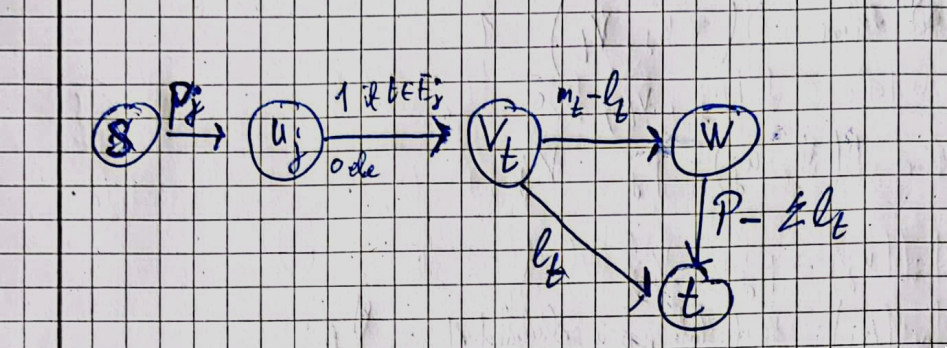
\includegraphics[width=0.6\textwidth]{graphics/sketches/flow_network.png}\label{fig:flow}
  \caption{The Flow-Network for checking feasibility of a scheduling instance with lower and upper bounds $l_t$ and $m_t$ for the number of busy processors at $t$.}
\end{figure}

\todo{Ambiguity of $t$ used for time slots and sink in flow-network: Use $\alpha$-$\omega$ flow}

\begin{lemma}\label{lemma:flow_feasibility}
  There exists a feasible solution to a scheduling instance with lower and upper bounds $l_t, m_t$ if and only if the maximum $s$-$t$ flow in the corresponding flow network depicted in Figure~\ref{fig:flow} has value $P$.
\end{lemma}
\begin{proof}
  Let $f$ be a $s$-$t$ flow of value $|f| = P$.
  We construct a feasbile schedule from $f$ respecting the lower and upper bounds given by $l_t$ and $m_t$.
  For every $j \in J$ and  $t \in T$, if $f(u_j, v_t) = 1$, then schedule $j$ at slot $t$ on the lowest-numbered processor not scheduling some other job.
  Since $|f| = P$ and the capacity $c(\{s\}, V \setminus \{s\}) = P$, we have $f_{in}(u_j) = p_j$ for every $j \in J$.
  Hence $f_{out}(u_j) = \sum_{t \in E_j} f_{in}(v_t) = p_j$.
  Hence every job $j$ is scheduled in $p_j$ distinct time slots within its execution interval.

  The schedule respects the upper bounds $m_t$, since $c(v_t, w) + c(v_t, t) \leq m_t - l_t + l_t$ and hence for every $t$ at most $m_t$ jobs are scheduled at $t$.

  The schedule respects the lower bounds $l_t$, since
  $c(V \setminus \{t\}, \{t\}) = P$ and hence
  $f(v_t, t) = l_t$ for every slot $t$.
  By flow conservation we then have $f_{in}(v_t) \geq l_t$ which implies that at least $l_t$ jobs are scheduled at every slot $t$.

  For the other direction consider a feasible schedule respecting the lower and upper bounds $l_t, m_t$.
  We construct a flow $f$ of value $P$ and show that it is maximal.

  If $j$ is scheduled at slot $t$ and hence $t \in E_j$,
  define $f(u_j, v_t) = 1$, otherwise $f(u_j, v_t) = 0$.
  Define $f(s, u_j) = p_j$ for every $j \in J$.
  Hence we have $f_{in}(u_j) = p_j$
  and $f_{out}(u_j)$ must be  $p_j$ since this corresponds to the number of distinct time slots in which $j$ is scheduled.
  Define $f(v_t, t) = l_t$ for every slot $t$.
  Define $f(v_t, w) = f_{in}(v_t) - l_t$.
  We have $f(v_t, w) \leq m_t - l_t$ since $f_{in}(v_t)$ corresponds to the number $\vol(t)$ of jobs scheduled at $t$, which is at most $m_t$.
  We also have $f_{out}(v_t) = f_{in}(v_t) - l_t + l_t = f_{in}(v_t)$.

  Define $f(w, t) = P - \sum_{t \in T} l_t$.
  Then $f_{in}(w) = \sum_{t \in T} f_{in}(v_t) - l_t
  = \sum_{t \in T} \vol(t) - \sum_{t \in T} l_t$.
  Since the schedule is feasible, we have $\sum_{t \in T} \vol(t) = P$ and finally the flow conservation $f_{in}(w) = P - \sum_{t \in T} l_t = f_{out}(w)$.

\end{proof}

\begin{theorem}
  Given a feasible problem instance, algorithm $\PLTR$ constructs a feasible schedule.
\end{theorem}
\begin{proof}
  By definition of subroutines $\keepidle$ and $\keepbusy$, $\PLTR$ only modifies the upper and lower bounds $m_t, l_t$ for the number of busy processors such that the resulting instance of \emph{power-down scheduling with lower and upper bounds} remains feasible.
  The correctness of the algorithm then follows from the correctness of the flow-calculation for checking feasibility, which is implied by Lemma~\ref{lemma:flow_feasibility}.
\end{proof}

\section{Structure of the PLTR-Schedule}
\subsection{Preliminary Definitions}
\begin{definition}
  Let $S$ be a schedule.
  The \emph{volume} $\vol_S(j, Q)$ of a job $j \in J$ in a set $Q \subseteq T$ of time slots is the number of time slots of $Q$ for which $j$ is scheduled at by $S$.
\end{definition}
\todo{Use just one definition environment for all volume definitions?}
\begin{definition}
  We define the \emph{forced volume} $\fv(j, Q)$ of job $j \in J$ in a set $Q \subseteq T$ of time slots as the minimum number of time slots of $Q$ for which $j$ has to be scheduled in every feasible schedule, i.e.
  \begin{align}
    \fv(j, Q) \coloneqq \max\{0; p_j - |E_j \setminus Q|\} \text{.}
  \end{align}
\end{definition}
\begin{definition}
  We define the \emph{unnecessary volume} $\uv_S(j, Q)$ of job $j \in J$ in a set $Q \subseteq T$ of time slots as the amount of volume which does not have to scheduled during $Q$, i.e.
  \begin{align}
    \uv_S(j, Q) \coloneqq \vol_S(j, Q) - \fv(j,Q)\text{.}
  \end{align}
\end{definition}
\begin{definition}
  We define the \emph{possible volume} $\pv(j, Q)$ of job $j \in J$ in a set $Q \subseteq T$ of time slots as the maximum amount of volume which $j$ can be feasibly scheduled in $Q$, i.e.
  \begin{align}
    \pv(j, Q) \coloneqq \min\{ p_j, | E_j \cap Q | \} \text{.}
  \end{align}
\end{definition}
%\begin{definition}
%  We define the \emph{space $\spac_S(j, Q)$ of job $j \in J$ in a set $Q \subseteq T$ for schedule $S$} as the number of additional time slots, which $j$ can be scheduled in $Q$, i.e.\
%  \begin{align}
%    \spac_S(j, Q) \coloneqq \pv(j, Q) - \vol_S(j, Q) \text{.}
%  \end{align}
%\end{definition}
Since the corresponding schedule $S$ will always be clear from context, we drop the subscript for $\vol, \uv$ and $\spac$.
We extend our volume definitions to single timeslots $t\in T$ and to sets $J' \subseteq J$ of jobs by summing over all $j \in J'$, i.e.
\begin{align}
  \vol(J', Q) &\coloneqq \sum_{j \in J'} \vol(j, Q)\text{,}
  \\
  \vol(t) &\coloneqq \vol(J, \{t\})\text{.}
\end{align}
If the first parameter is dropped, we refer to the whole set $J$, i.e.\ $\vol(Q) \coloneqq \vol(J, Q)$.
Clearly we have for every feasible schedule, every $Q \subseteq T, j \in J$ that $\fv(j, Q) \leq \vol(j, Q) \leq \pv(j, Q)$.

\begin{definition}
  We define the \emph{density} $\phi(Q)$ for a set $Q \subseteq T$ as the average amount of processing volume which has to be completed in every slot of $Q$, i.e.
  $\phi(Q) \coloneqq \fv(J, Q) / |Q|$.
  We also define $\hat \phi(Q) \coloneqq \max_{Q' \subseteq Q} \phi(Q')$.
\end{definition}
If $\hat \phi(Q) > k - 1$, then clearly at least $k$ processors are required in some time slot $t \in Q$ for every feasible schedule.
\begin{definition}
  We define the \emph{deficiency $\opdef(Q)$ of a set $Q \subseteq T$ of time slots} as the difference between the amount of volume which has to be completed in $Q$ and the processing capacity available in $Q$, i.e. $\opdef(Q) \coloneqq \fv(Q) - \sum_{t \in Q} m_t$.
\end{definition}
\begin{definition}
  We define the \emph{excess $\exc(Q)$ of a set $Q \subseteq T$ of time slots} as the difference between the processor utilization required in $Q$ and the amount of processing volume available in $Q$, i.e. $\exc(Q) \coloneqq \sum_{t \in Q} l_t - \pv(Q)$.
\end{definition}
\subsection{Critical set of time slots}
\begin{lemma}\label{lemma:cut}
  For every $s$-$t$ cut $(S, \bar S)$ in the network given in Figure~\ref{fig:flow} we have at least one of the following two lower bounds for the capacity $c(S)$ of the cut:
  $c(S) \geq P - \opdef(Q(S))$ or $c(S) \geq P - \exc(Q(\bar S))$, where $Q(S) \coloneqq \{ t \mid v_t \in S \}$.
\end{lemma}
\begin{proof}
  Let $(S, \bar S)$ be an $s$-$t$ cut, let $J(S) \coloneqq \{j \mid u_j \in S\}$.
  We consider the contribution of every node of $S$ to the capacity $c(S)$ of the cut.
  First consider the case that $w \notin S$.
  \begin{itemize}
    \item Node $s$: $\sum_{j \in J(\bar S)} p_j$.
    \item Node $u_j$: $|\{v_t \in \bar S \mid t \in E_j\}| = | E_j \setminus Q(S) | \geq p_j - \fv(j, Q(S))$
    \item Node $v_t$: $l_t + m_t - l_t = m_t$
  \end{itemize}
  The inequality for node $u_j$ follows since $\fv(j, Q(S)) = \max \{0, p_j - |E_j \setminus Q(S)| \}$.
  In total, we can bound the capacity from below with
  \begin{align}
    c(S) &\geq \sum_{j \in J(\bar S)} p_j + \sum_{j \in J(S)} p_j - \fv(j, Q(S)) + \sum_{t \in Q(S)} m_t
    \\ &= P - \fv(J(S), Q(S)) + \sum_{t \in Q(S)} m_t
    \\ &\geq P - \opdef(Q(S))\text{.}
  \end{align}
  If $w \in S$, we have the following contributions of nodes in $S$:
  \begin{itemize}
    \item Node $s$: $\sum_{j \in J(\bar S)} p_j \geq \pv(J(\bar S), Q(\bar S))$.
    \item Node $u_j$: $| E_j \setminus Q(S) |
      = | E_j \cap Q(\bar S)| \geq \pv(j, Q(\bar S))$
    \item Node $v_t$: $l_t$
    \item Node $w$: $P - \sum_{t \in T} l_t$
  \end{itemize}
  In total, we obtain the lower bound
  \begin{align}
    c(S) &\geq P + \pv(Q(\bar S))
    - \sum_{t \in Q(\bar S)} l_t
    \\ &= P - \exc(Q(\bar S)) \text{.}
  \end{align}

\end{proof}

\begin{lemma}\label{lemma:feasibility}
  An instance of power-down scheduling with lower and upper bounds is feasible if and only if $\opdef(Q) \leq 0$ and $\exc(Q) \leq 0$ for every $Q \subseteq T$.
\end{lemma}
\begin{proof}
  If $\opdef(Q) > 0$ for some $Q$, then some upper bound $m_t$ cannot be met.
  If $\exc(Q) > 0$ for some $Q$, then some lower bound $l_t$ cannot be met.
  For the direction from right to left, consider an infeasible scheduling instance with lower and upper bounds.
  By Lemma~\ref{lemma:flow_feasibility} we have that the maximum flow $f$ for this instance has value $|f| < P$.
  Hence, there must be a $s$-$t$ cut $(S, \bar S)$ of capacity $c(S) < P$.
  Lemma~\ref{lemma:cut} now implies that $\opdef(Q(S)) > 0$ or $\exc(Q(\bar S)) > 0$.
\end{proof}
\begin{definition}
  A time slot $t \in T$ is called \emph{activation of processor $k \in [m]$} if processor $k$ is idle at $t-1$ and busy at $t$.
  A time slot $t \in T$ is just called \emph{activation} if it is an activation of processor $k$ for some $k \in [m]$.
\end{definition}
The following lemma provides the crucial structure required for the proof of the approximation guarantee.
Intuitively, it states that for every activation $t$ of processor $k$ in the schedule $S_{\pltr}$ returned by $\PLTR$, there must be some set $Q$ of timeslots during which an activation of processor $k$ is necessary in every feasible schedule.
\begin{lemma}\label{lemma:critical}
  For every time slot $t \in T$ for which some processor $k \in [m]$ becomes busy in $S_{\pltr}$, there exists a set $Q \subseteq T$ of time slots with $t \in Q, $
  \begin{align}
    \fv(Q) &= \vol(Q) \text{,}\\
    \vol(t') &\geq k-1 &~\text{for all}~t' \in Q~\text{and}\\
    \vol(t') &\geq k &~\text{for all}~t' \in Q~\text{with}~t' \geq t \text{.}
  \end{align}
\end{lemma}
\begin{proof}
  Suppose for contradiction that there is some activation $t \in T$ of processor $k \in [m]$ and no such $Q$ exists for $t$.
  We show that $\PLTR$ would have extended the idle interval on processor $k$ which ends at $t$.
  Consider the step in $\PLTR$ when $t$ was the result of $\keepidle$ on processor $k$ and the corresponding lower and upper bounds $m_{t'}, l_{t'}$ for $t' \in T$ right after the calculation of $t$ with the corresponding update of the bounds by $\keepidle$.
  We modify the bounds by decreasing $m_t$ by $1$.
  Note that at this point $m_{t'} \geq k$ for every $t' > t$ and $m_{t'} \geq k - 1$ for every $t'$.

  Consider $Q \subseteq T$ such that $t \in Q$ and $\fv(Q) < \vol(Q)$.
  Before our decrement of $m_t$ we had $m_Q \coloneqq \sum_{t' \in Q} m_{t'} \geq \vol(Q) > \fv(Q)$.
  The inequality $m_Q \geq \vol(Q)$ here follows since the upper bounds $m_{t'}$ are monotonically decreasing during $\PLTR$.
  Since our modification decreases $m_Q$ by at most $1$, we hence still have $m_Q \geq \fv(Q)$ after the decrement of $m_t$.

  Consider $Q \subseteq T$ such that $t \in Q$ and $\vol(t') < k - 1$ for some $t'$.
  At the step in $\PLTR$ considered by us, we hence have $m_{t'} \geq k - 1 > \vol(t')$.
  Before our decrement of $m_t$ we therefore have $m_Q > \vol(Q) \geq \fv(Q)$, which implies $m_Q \geq \fv(Q)$ after the decrement.

  Finally, consider $Q \subseteq T$ such that $t \in Q$ and $\vol(t') < k$ for some $t' > t$.
  At the step in $\PLTR$ considered by us, we again have $m_{t'} \geq k > \vol(t')$, which implies $m_Q \geq \fv(Q)$ after our decrement of $m_t$.
  In summary, if for $t$ no $Q$ exists as characterized in the proposition, the activation of processor $k$ at $t$ could not have been the result of $\keepidle$ on processor $k$.
\end{proof}

\begin{definition}
  We call such $Q \subseteq T$ for activations $t$ of processor $k$ characterized by Lemma~\ref{lemma:critical} \emph{tight set $Q_t$ over activation $t$ of processor $k$}.
\end{definition}

\begin{definition}
  A \emph{critical set $C_t \subseteq T$ over an activation $t$} is the maximum of the set of tight sets $Q_t$ over activation $t$ in regard to the density $\phi$, i.e.
  \begin{align}
    C_t \coloneqq \argmax \{ \phi(Q) \mid Q \subseteq T~\text{is tight set over}~t \} \text{.}
  \end{align}
  As the set of these critical sets $C_t$ for fixed $t$ is closed under union, we take $C_t$ to be the inclusion-maximal critical set over activation $t$ for the sake of uniqueness.
\end{definition}

\subsection{Definitions based on critical sets}
\begin{definition}
  \todo{Use $\succeq$ instead of $\preceq$ here}
  We define a total order $\succeq$ on the set of critical sets $C_t$ across all activations $t$.
  For activations $t, t' \in T$ of processors $k$ and $k'$ respectively, we define $C_t \succeq C_{t'}$ if and only if $k > k'$ or $k = k'$ and $t \leq t'$.
  In other words, $\succeq$ defines the same order in which $\PLTR$ calculates the activations: from Top-Left to Bottom-Right.
  Equality in regard to $\succeq$ is denoted with $\sim$.
\end{definition}
\begin{definition}
  Let $\rank: \{C_t\} \rightarrow \mathbb{N}$ be a mapping to the natural numbers corresponding to $\succeq$, i.e.
  \begin{align}
    \rank(C_t) \geq \rank(C_{t'})
    \iff
    C_t \succeq C_{t'} \text{.}
  \end{align}
\end{definition}
\begin{definition}
  Let $\crit: \{C_t\} \rightarrow [m]$ be a mapping to the processors s.t.
  \begin{align}
    \crit(C_t) = c
    \iff
    c~\text{is the highest processor activated at}~t \text{.}
  \end{align}
\end{definition}
\begin{definition}
  We extend these definitions \todo{welche? rank?} to general time slots $t \in T$ as follows.
  \begin{align}
    \rank(t) \coloneqq
    \begin{cases}
      \max \{\rank(C) \mid t \in C \}
      & \text{if}~t \in C~\text{for some critical set}~C
      \\0
      & \text{otherwise}
    \end{cases}
  \end{align}
  \begin{align}
    \crit(t) \coloneqq
    \begin{cases}
      \max \{\crit(C) \mid t \in C \}
      & \text{if}~t \in C~\text{for some critical set}~C
      \\0
      & \text{otherwise}
    \end{cases}
  \end{align}
  We also extend the definitions to intervals $D \subseteq T$ with
  \begin{align}
    \rank(D) &\coloneqq \max \{ \rank(t) \mid t \in D \} \text{,}
    \\ \crit(D) &\coloneqq \max \{ \rank(t) \mid t \in D \} \text{.}
  \end{align}
\end{definition}
\begin{definition}
  Let $C$ be a critical set. A nonempty interval $V \subseteq T$ is a \emph{valley of $\rank(C)$} if $C \sim V$ and $V$ is inclusion maximal.
  Let $C_1, \ldots, C_l$ be the intervals contained in $C$.
  A nonempty interval $V$ is a \emph{valley of $C$} if $V$ is exactly the interval between $C_{a}$ and $C_{a+1}$ for some $a < l$, i.e. $V = [\max C_a + 1, \min C_{a+1} - 1]$.
\end{definition}
\begin{definition}
  \todo{Think about using a different term than \emph{to span} here, e.g.\ \emph{to partially span}.}
  For a critical set $C$, an interval $D$ \emph{spans} $C$ if $D \cap C$ contains only full subintervals of $C$ and at least one subinterval of $C$.
  The \emph{left valley} $V_l$ of $C$ and an interval $D$ spanning $C$ is the valley of $C$ ending at $\min (C \cap D) - 1$ if such a valley of $C$ exists.
  Symmetrically, the \emph{right valley} $V_r$ of $C$ and an interval $D$ spanning $C$ is the valley of $C$ starting at $\max (C \cap D) + 1$ if such a valley of $C$ exists.
\end{definition}

\begin{definition}
  \todo{Use $J(V)$ everywhere to not have double subscripts later?}
  For a valley $V$, we define the jobs $J_V \subseteq J$ as all jobs which are scheduled by $S_{\pltr}$ in every $t \in V$.
\end{definition}

\begin{lemma}\label{lemma:valley}
  For every critical set $C$ with $c \coloneqq \crit(C)$, every interval $D \subseteq T$ spanning $C$:
  if $\phi(C \cap D) \leq c - \delta$ for some $\delta \in \mathbb{N}$, then the left valley $V_l$ or the right valley $V_r$ of $C$ and $D$ is defined and $|J_{V_l}| + |J_{V_r}| \geq \delta$, where we take $|J_V| \coloneqq 0$ if $V$ is not defined.
\end{lemma}
\todo{Provide a rough visual sketch here}
\begin{proof}
  \todo{Make math more readable in this whole proof, e.g.\ by using fractions and display math, by replacing division by multiplication, or by introducing $l \coloneq |C \cap D|$}
  By choice of $C$ as critical set with $c = \crit(C)$ we have $\vol(C \cap D) \geq (c-1) \cdot |C \cap D|$.
  If this inequality is fulfilled strictly, i.e.\ if
  $\vol(C \cap D) > (c-1) \cdot |C \cap D|$, then with the premise
  $\fv(C \cap D) / |C \cap D| \leq c - \delta$ we directly get $\uv(C \cap D) / |C \cap D| > \delta - 1$.
  This implies that there are at least $\delta$ jobs $j$ scheduled in $C \cap D$ with $\uv(j, C \cap D) > 0$.
  Such jobs can be scheduled in the part of $C$ not contained in $D$, i.e.\ we must have $E_j \cap (C \setminus D) \neq \emptyset$ and hence the left valley $V_l$ or the right valley $V_r$ of $C$ and $D$ must exist.
  These jobs must be contained in $J_{V_l}$ or $J_{V_r}$ since they are scheduled in $C$ and the schedule is feasible.

  If on the other hand we have equality, i.e.\ $\vol(C \cap D) = (c-1) \cdot |C \cap D|$, then let $t$ be the activation of processor $c$ for which $C$ is the critical set.
  Since $\vol(t) > c-1$, we must have $t \notin C \cap D$.
  By the same argument as before, we have that if $\fv(C \cap D) / |C \cap D| \leq c - \delta$, then $\uv(C \cap D) / |C \cap D| \geq \delta - 1$.
  Let $J' \coloneqq \{ j \in J \mid \uv(j, C \cap D) > 0 \}$.
  Clearly $|J'| \geq \delta - 1$.
  If this lower bound is fulfilled with equality, every $j \in J'$ must be scheduled in every time slot of $C \cap D$.
  Now suppose for contradiction that all jobs $j$ scheduled during $C$ which are not contained in $J'$ have $E_j \cap C \cap D = \emptyset$.
  %Now suppose for contradiction that there is no job $j$ scheduled in $C \setminus D$ with $
  %Now suppose that there is no job $j$ scheduled in $C$ such that $\spac(j, C \cap D) > 0$.
  Then $\fv(C \setminus D) = \vol(C \setminus D)$ and
  we get $\phi(C \setminus D) > \phi(C)$ since by case assumption $\vol(C \cap D) = (c-1) \cdot |C \cap D|$.
  In conclusion, $C \setminus D$ is still a tight set over $t$ but has higher density than $C$, contradicting the choice of $C$.
  Therefore, there must exist a job $j \notin J'$ scheduled in $C$ which can be scheduled $C \cap D$.

  In total, we have at least $\delta$ jobs scheduled in $C$ with an execution interval intersecting both $C \setminus D$ and $C \cap D$.
  This implies that the left valley $V_l$ or the right valley $V_r$ of $C$ and $D$ exists and that at least $\delta$ jobs are contained in $J_{V_l}$ or $J_{V_r}$.
\end{proof}

\section{Modification of our Schedule}
We modify the schedule $S_{\pltr}$ returned by $\PLTR$ in two steps.
The first step augments specific processors with auxiliary busy slots such that in every critical set $C$ at least the first $\crit(C)$ processors are busy all the time.
For the single processor Left-to-Right algorithm, the crucial property for the approximation guarantee is that every idle interval of $S_{\opt}$ can intersect at most $2$ distinct idle intervals of the schedule returned by Left-to-Right.
The second modification step of $S_{\pltr}$ is more involved and establishes this crucial property on every processor $k \in [m]$ by making use of Lemma~\ref{lemma:valley}.
More specificially, it will establish that $\hat \phi(A) > k - 1$ for every $\busy$ interval $A$ on processor $k$, i.e.\ that every feasible schedule requires $k$ busy processors at some point during $A$.

These modification steps are only done for the sake of the analysis of the original schedule $S_{\pltr}$ and are not part of the algorithm.
By making sure that the modifications cannot decrease the costs of our schedule, we get an upper bound for the costs of $S_{\pltr}$.

\subsection{Augmentation}
\todo{Make this into a proper definition of $S_{\aug}$?}
We transform $S_{\pltr}$ into the \emph{augmented schedule $S_{\aug}$} by adding for every $t$ with $k \coloneqq \crit(t) \geq 2$ and $\vol(t) = k-1$ an auxiliary busy slot on processor $k$.
No job is scheduled in this auxiliary busy slot on processor $k$ and it does also not count towards the volume of this slot.
It merely forces processor $k$ to be in the on-state at time $k$ and allows us to keep thinking in terms of $\idle$ and $\busy$ intervals in our analysis of the costs.

\begin{lemma}\label{lemma:augmented}
  In $S_{\aug}$ processors $1, \ldots, \crit(t)$ are busy in every slot $t \in T$ with $\crit(t) \geq 2$.
\end{lemma}
\begin{proof}
  The property directly follows from our choice of the critical sets, the definition of $\crit(t)$ and the construction of $S_{\aug}$.
\end{proof}

\subsection{Realignment}
The intuition of the realignment of $S_{\aug}$ is the following.
Lemma~\ref{lemma:augmented} guarantees us that every busy interval $A$ on processor $k$ spans the critical set $C$ with $C \sim A$.
It also guarantees that the left and right valley $V_l, V_r$ of $C$ and $A$ do not end within an idle interval on processor $k$, provided that they are defined.
Lemma~\ref{lemma:valley} in turn guarantees us that if the density of $A$ does not guarantee that $S_{\opt}$ has to use processor $k$ during $A$, i.e.\ if $\hat \phi(A) \leq k - 1$, then $V_l$ or $V_r$ is defined and there is some $j$ scheduled in every slot of $V_l$ or $V_r$.
Let $V$ be the corresponding left or right valley of $C$ and $D$ for which such a job exists.
Instead of scheduling this job on the processors below $k$, we can schdule the job on processor $k$ in idle time slots during $V$ instead of the lower processors, merging the busy interval $A$ with at least one neighbouring busy interval on processor $k$.
In the definition of the realignment, we will call this process of filling the idle slots during $V$ on processor $k$ closing of valley $V$ on processor $k$.

The crucial part is making sure that this realignment continues to be possible whenever we have a busy interval with a density which is too small.
For this purpose, we go through the busy intervals on each processor in the order of their rank, i.e.\ in the order of $\succeq$.
We also allow every job to be used twice for the realignment by introducing further auxiliary busy slots (for an interval $D$ spanning the critical set $C$, both the right and the left valley might be closed in the worst case).
This allows us to maintain the Invariants of Lemma~\ref{lemma:invariant} analogous to Lemma~\ref{lemma:augmented} and Lemma~\ref{lemma:valley} during the realignment process.



\begin{algorithm}[H]
  \caption{Realignment of $S_{\aug}$}\label{alg:real}
\begin{algorithmic}
  \State{$\res(V) \gets 2 |J_V|$ for every valley $V$}
  \For{$k \gets m$ \textrm{to} $1$}
    \State{\Call{$\fillop$}{$k, T$}}
    \State{$\res(V) \gets \res(V) - 1$ for every valley $V$
    s.t.\ some $V'$ with $V' \cap V \neq \emptyset$ was closed on processor $k$}
  \EndFor{}
\end{algorithmic}
\end{algorithm}

\todo{Explicitly define \emph{valley $V$ having been closed on processor $k$} as $\close(k, V)$ having been called.}

\begin{algorithm}[H]
  \caption{Subroutines for the Realignment of $S_{\aug}$}\label{alg:real_suppl}
\begin{algorithmic}
  \Function{$\fillop$}{$k, V$}
    \If{$\crit(V) \leq 1$}
      \State{\Return{}}
    \EndIf{}
    \State{let $C$ be the critical set s.t.\ $C \sim V$}
    \While{exists busy interval $A \subseteq V$ on processor $k$
    with $A \sim V$ and $\hat \phi(A) \leq k - 1$}
      \State{let $V_l, V_r$ be the left and right valley for $C$ and interval $A$ (if $A$ spans $C$)}
      \If{$V_l$ exists and $\res(V_l) > 0$}
        \State{\Call{$\close$}{$k, V_l$}}
      \ElsIf{$V_r$ exists and $\res(V_r) > 0$}
        \State{\Call{$\close$}{$k, V_r$}}
      \EndIf{}
    \EndWhile{}
    \For{every valley $V' \subseteq V$ of $C$ which has not been closed on $k$}
      \State{\Call{$\fillop$}{$k, V'$}}
    \EndFor{}
  \EndFunction{}

  \Function{$\close$}{$k, V$}
    \For{every $t \in V$ which is idle on processor $k$}
      \If{processors $1, \ldots, k-1$ idle at $t$}
        \State{introduce new auxiliary busy slot on processor $k$ at time $t$}
      \Else{}
        \State{move busy slot at time $t$ of highest processor
        among $1, \ldots, k-1$ to processor $k$ at $t$}
      \EndIf{}
    \EndFor{}
  \EndFunction{}
\end{algorithmic}
\end{algorithm}

\subsection{Invariants for Realignment}
\begin{lemma}\label{lemma:invariant}
  For an arbitrary step during the realignment of $S_{\aug}$ and a valley $V \subseteq T$, let $k_V$ be the highest processor such that
  \begin{itemize}
    \item
      processor $k_V$ is not fully filled yet, i.e.\ $\fillop(k_V, T)$ has not yet returned,
    \item
      no $V' \supseteq V$ has been closed on $k_V$ so far and
    \item
      there is a (full) busy interval $A \subseteq V$ on processor $k_V$.
  \end{itemize}
  We take $k_V \coloneqq 0$ if no such processor exists.
  At every step in realignment of $S_{\aug}$ the following invariants hold.
  \begin{enumerate}
    \item
      If $\phi(C \cap D) \leq k_V - \delta$ for some $\delta \in \mathbb{N}$ and some interval $D \subseteq T$ spanning $C$, then the left valley $V_l$ or the right valley $V_r$ of $C, D$ exists and $\res(V_l) + \res(V_r) \geq 2 \delta$.
    \item
      For every $t \in C \cap V$, processors $1, \ldots, k_V$ are busy at $t$.
    \item
      Every busy interval $A \subseteq V$ on processor $k_V$ with $A \sim V$ spans $C$.
  \end{enumerate}
\end{lemma}
\begin{proof}
  We show properties 1 and 2 via structural induction on the realigned schedule $S_{\real}$.
  Then we show that invariant 2 implies invariant 3.
  For the induction base, consider $S_{\aug}$ and let $V$ be an arbitrary valley in $S_{\aug}$ and $C$ the critical set with $C \sim V, \crit(V) \coloneqq c$.

  We have $k_V \leq c$, otherwise $V$ contains a full busy interval on processor $k_V > c$ and hence also an activation $t \in V$ of processor $k_V$, which by construction of $S_{\aug}$ would have $\crit(t) = k_V > c$. This is a direct contradiction to $\crit(V) = \max_{t \in V} \crit(t) = c$.

  The second invariant now follows since by construction of $S_{\aug}$ and our choice of $C$ we have for every $t \in C$ that processors $1, \ldots, k_V, \ldots, c$ are busy at $t$.

  For the first invariant, let $D$ be an interval spanning $C$ with $\phi(C \cap D) \leq k_V - \delta$ for some $\delta \in \mathbb{N}$.
  With $k_V \leq c$ we get $\phi(C \cap D) \leq c - \delta$ and hence by Lemma~\ref{lemma:valley}, we have that the left valley $V_l$ or the right valley $V_r$ of $C$ and $D$ exists and $|J_{V_l}| + |J_{V_r}| \geq \delta$.
  With the initial definition of $\res(V)$ we get the desired lower bound of $\res(V_l) + \res(V_r) \geq 2 \delta$.

  Now suppose that invariants 1 and 2 hold at all steps of the realignment up to a specific next step.
  Let $V$ again be an arbitrary valley of $\crit(V) \geq 2$ and $k$ the processor currently being filled.
  Let furthermore $k_V, k'_V$ be the critical processor for $V$ before and after, respectively, the next step in the realignment.
  We consider four cases for the next step in the realignment.

  %\begin{enumerate}
  %  \item
  %    Some $V' \supseteq V$ is closed on processor $k$.
  %  \item
  %    Some $V' \subset V$ is closed on processor $k$.
  %  \item
  %    Some $V'$ with $V' \cap V = \emptyset$ is closed on processor $k$.
  %  \item
  %    The call to $\fillop(k, T)$ returns and $\res(V')$ is decreased by 1 for every $V'$ such that some valley intersecting $V'$ has been closed during $\fillop(k, T)$.
  %\end{enumerate}
  \paragraph{Case 1:}
      Some $V' \supseteq V$ is closed on processor $k$.
      Then no valley $W$ intersecting $V$ has been closed so far on $k$.
      Also, since $\close$ only moves the busy slot of the highest busy processor below $k$, we know that the stair property \todo{define stair property} holds within $V$ on processors $1, \ldots, k$.
      We show that the closing of $V'$ on $k$ reduces the critical processor of $V$ by at least $1$, i.e. $k'_V \leq k_V - 1$.
      If $k_V = k$, then $V' \supseteq V$ is closed on processor $k_V$ and hence by definition we have $k'_V \leq k_V - 1$.
      If $k_V < k$, suppose for contradiction that $k_V \leq k'_V \leq k$, where $k'_V \leq k$ again by definition since $V' \subseteq V$ is closed on processor $k$.

      Let $A \subseteq V$ be a full busy interval on $k_V$ before the close of $V'$.
      We show that $A \subset V$, i.e.\ that there must be some $t \in V$ idle on $k_V$ before the close and hence by the stair-property processors $k_V, \ldots, k$ idle at $t$ before the close.
      If $V' \supseteq V$ is closed, clearly $V \subset T$ by the choice of $V_l$ and $V_r$ as valleys of some critical set in the realignment definition.
      Hence we know that $\min V - 1 \in T$ and $\max V + 1 \in T$.
      \todo{Double check if this is true (or if we only have one of the two guaranteed): Since $V$ must be valley \emph{of} some $C$, we should have both $0 \notin V$ and $d^* \notin V$.}
      We show that $t \coloneqq \min V - 1$ must be busy on $k_V$ before the close.
      Let $W \supseteq V$ be the valley with $W \sim t$ and $t \in W$.
      We know that $W \supseteq V$ since $W \sim t \succ V$ since $V$ is a valley.
      By our case assumption, no $W' \subseteq W$ can have been closed on processor $k$ so far.
      With $W \supseteq V$ and the definition of $k_W$ we get $k_W \geq k_V$, where $k_W$ is the critical processor of $W$ before the close.
      Our induction hypothesis now implies that processors $1, \ldots, k_V, \ldots, k_W$ are busy at $t$ before the close.
      For $A \subseteq V$ to be a (full) busy interval on $k_V$ before the close, we hence must have $\min V \notin A$.
      We know by definition of the realignment and function $\close$, that for every $k'$ with $k_V \leq k' < k$ and every $t \in V$:
      \begin{itemize}
        \item
          If $t$ was idle on $k'$ before the close, then $t$ is still idle on $k'$ after the close (definition of $\close$, $k' < k$).
        \item
          If $t$ was idle on $k_V$ before the close, then $t$ was idle on $k'$ before (stair-property) and hence $t$ is still idle on $k'$ after the close.
        \item
          If $t$ was part of full a busy interval $A \subset V$ on $k_V$ before the close, then $t$ was idle on $k_V + 1$ before the close (choice of $k_V$).
          Hence $t$ was idle on $k$ before (stair-property) and hence $t$ is idle on $k_V$ after the close.
      \end{itemize}
      Taken together, for $t \in V$ to be busy on $k'$ after the close, $t$ must have been busy on $k'$ before the close (definition $\close, k' < k$) and $t$ cannot have been part of a full busy interval $A \subseteq V$.
      Hence $t \in A$ for some \todo{properly define partial busy intervals} \emph{partial} busy interval $A \subseteq V$ on $k'$ before the close.
      For $A' \subseteq V$ to be a full busy interval on $k'_V$ after the close (with $k_V \leq k'_V < k$), we must have $A' \subseteq A$.
      \begin{figure}[H]
        \centering
        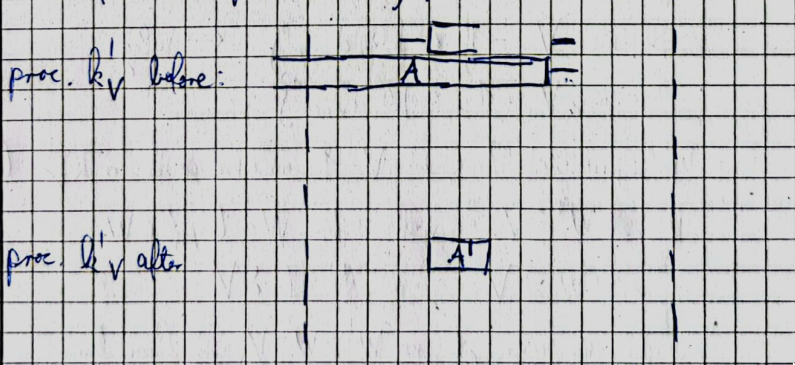
\includegraphics[width=0.5\textwidth]{graphics/sketches/invariant_case1.png}\label{fig:invariant_case1}
        \caption{The situation for case $1$ in Lemma~\ref{lemma:invariant}.}
      \end{figure}
      Hence there must have been a busy interval $A'' \subseteq [\min A', \max A]$ on processor $k'_V + 1 > k_V$ before the close, which contradicts the definition of $k_V < k$.
      In conclusion, we have $k'_V \leq k_V - 1$ which allows us to prove our invariants 1 and 2.
      If $\phi(C \cap D) \leq k'_{V} - \delta$ for some $\delta \in \mathbb{N}$ and some interval $D$ spanning $C$, then $\phi(C \cap D) \leq k_V - (\delta + 1)$ and hence by induction hypothesis the left valley $V_l$ or the right valley $V_r$ for $C, D$ exists and $\res(V_l) + \res(V_r) \leq 2 (\delta + 1)$ both before and after the close.
      Our induction hypothesis also implies that for every $t \in C \cap V$ processors $1, \ldots, k_V$ are busy before the close.
      Since at most the uppermost busy slot is moved by $\close$, after the close of $V'$ we still have processors $1, \ldots, k_V - 1 \geq k'_V$ busy.

  \paragraph{Case 2:}
      Some $V' \subset V$ is closed on processor $k$.
      Again, no $V'' \supseteq V$ can have been close on processor $k$ so far.
      We show that $k_V = k \geq k'_V$, i.e.\ that the critical processor of $V$ before the close of $V'$ is the processor currently being filled.
      Let $W$ be the valley for which $V'$ is closed, i.e.\ $V'$ is closed during $\fillop(k, W)$.
      We must have $W \supset V'$ and therefore no $W' \supseteq W$ has been closed on $k$ so far.
      Also, for $V'$ to be closed in $\fillop(k, W)$, there must be some busy interval $A \subseteq W$ on $k$ before the close, hence $k_W = k$.
      Since $V' \subset V$ and $V' \subset W$, $V$ and $W$ intersect ($V' \neq \emptyset$ by definition of $V'$ as valley).
      If $V \prec W$, then by choice of $V'$ as valley of $C_W$
      \todo{introduce this notation for critical set $C_V$ of valley $V$, i.e.\ $C_V \sim V$.}
      we must have $V \subseteq V'$, which contradicts our case assumption.
      Therefore $V \succeq W$ and $V \supseteq W$ implying $k_V \leq k_W = k$ and since processor $k+1$ is already filled before the close we have $k_V = k \geq k'_V$.

      For invariant 1, again let $\phi(C \cap D) \leq k'_V - \delta \leq k_V - \delta$ for some $\delta \in \mathbb{N}$ and some interval $D$ spanning $C$.
      Our induction hypothesis implies that the left valley $V_l$ or the right valley $V_r$ of $C, D$ exists and that both before and after the close we have $\res(V_l) + \res(V_r) \geq 2 \delta$.

      For invariant 2, observe that $V' \cap C = \emptyset$ since $V' \prec C$ by our case assumption.
      Our invariant 2 now directly follows from the induction hypothesis and $k'_V \leq k_V$.


  \paragraph{Case 3:}
      Some $V'$ with $V' \cap V = \emptyset$ is closed on processor $k$.
      We first show that $\min V - 1 \notin V'$ and symmetrically $\max V + 1 \notin V'$.
      Consider $t \coloneqq \min V - 1$.
      We know $t \in T$ since $V'$ is valley of some critical set.
      By choice of $V$ and $t$ we must have $t \succ V$.
      If $t \in V'$, we would have $V' \succ V$ and hence $V' \supseteq V$, which contradicts our case assumption.
      Symmetrically, we know that $\max V + 1 \notin V'$.
      Therefore the close of $V'$ does not modify the schedule within $[\min V - 1, \max V + 1]$, implying that no partial busy interval in $V$ before the close can become a full busy interval.
      In summary we have $k_V = k'_V$ and invariants 1 and 2 follow as in case 2.

  \paragraph{Case 4:}
      The call to $\fillop(k, T)$ returns and $\res(V')$ is decreased by 1 for every $V'$ such that some valley intersecting $V'$ has been closed during $\fillop(k, T)$.
      First observe that the schedule itself does not change by this step but processor $k$ is now fully filled, which implies $k'_V \leq k_V$.
      Invariant 2 then follows directly from the induction hypothesis.

      We consider two subcases.
      If during $\fillop(k, T)$, no valley $V'$ intersecting $V$ was closed on $k$, then $\res(V)$ does not change and Invariant 1 follows from the induction hypothesis and $k'_V \leq k_V$.
      If on the other hand some valley $V'$ intersecting $V$ was closed on $k$ during $\fillop(k, T)$, then $\res(V)$ is decresed by $1$ to $\res'(V) \coloneqq \res(V) - 1$.
      As seen in cases 1 to 3, $k_V$ decreases monotonically during $\fillop(k, T)$.
      Consider the schedule right before the first valley $V'$ intersecting $V$ is closed on $k$.
      Let $k^0_V$ be the critical processor for $V$ at this point of the realignment and $k^1_V$ the critical processor right after $V'$ is closed.

      We have $k'_V \leq k^0_V - 1$:
      If $V' \supseteq V$, then as argued in case 1 $k^1_V \leq k^0_V - 1$ and hence $k'_V \leq k_V \leq k^1_V \leq k^0_V -1$.
      If $V' \subset V$, then as argued in case 2 we have $k^0_V = k$.
      Since $\fillop(k, T)$ returns in the next step of our case assumption, we have $k'_V \leq k - 1$ and hence $k'_V \leq k^0_V -1$.
      Invariant 2 now follows by our (strong) induction hypothesis.
      If $\phi(C \cap D) \leq k'_V - \delta$ then $\phi(C \cap D) \leq k^0_V - (\delta + 1)$ and hence the left valley $V_l$ or the right valley $V_r$ of $C, D$ exists and before the close $\res(V_l) + \res(V_r) \geq 2 (\delta + 1)$.
      Since $\res$ is decreased by at most $1$, we have after the close $\res'(V_l) + \res'(V_r) \geq 2 \delta$.

  We conclude by showing that Invariant 2 implies Invariant 3.
  Let $V$ be an arbitrary valley during the realignemnt of $S_{aug}$ and $A \subseteq V$ a busy interval on processor $k_V$ with $A \sim V$.
  Let $C$ be the critical set with $C \sim V$.
  Note that $A \sim V$ implies that $A$ intersects $C$.
  Assume for contradiction that $A$ does not span $C$.
  The $\min A$ is within subinterval of $C$ or symmetrically $\max A$ within subinterval of $C$.
  We assume the first case, i.e.\ $t\coloneqq \min A - 1 \in C$ and $\min A \in C$.
  The second case follows by symmetry.
  If $t \in V$, then time slot $t$ is busy on processor $k_V$ by Invariant 2.
  Therefore, $A$ cannot be a (full) busy interval on processor $k_V$, contradicting the choice of $A$.
  If $t = \min V-1$, then consider valley $W$ with $t \in W$ and $t \sim W$.
  We must have $W \supset V$, $W \succ V$ and $t \in C_W$.
  Therefore $k_W \geq k_V$ and Invariant 2 implies that $t = \min A - 1$ is busy on processor $k_V$, again contradicting the choice of $A$ as full busy interval on processor $k_V$.
\end{proof}

\begin{lemma}\label{lemma:s_real}
  The result $S_{\real}$ of the realignment of $S_{\aug}$ is defined.
\end{lemma}
\begin{proof}
  The Invariants in Lemma~\ref{lemma:invariant} imply that whenever we are inside the while-loop of $\fillop$, the corresponding busy interval $A$ indeed spans the corresponding critical set $C$ with $C \sim A$, hence $V_r$ or $V_l$ exists and there is suffcient $\res$ to close some valley.

  Since in the while-loop of $\fillop(k, V)$ the busy interval $A \subseteq V$ on $k_V$ always spans $C$ if $V \sim C$ (Invariant 3), the left valley $V_l$ and the right valley $V_r$ of the critical set $C$ and interval $A$ are properly defined.
  Also since $\phi(A) \leq k - 1$, Invariant 1 implies that $V_l$ or $V_r$ exists and that there is sufficient $\res$ such that one of the two valleys of $C$ is closed in this iteration.
  This reduces the number of idle intervals on processor $k$ by at least $1$, since Invariant 2 implies that $V_l$ or $V_r$ cannot end strictly within an idle interval on $k$.
  Hence all terms in the realignment are well defined and the realignment terminates.
\end{proof}

\begin{lemma}\label{lemma:phi_prop}
  For every processor $k \in [m]$, every busy interval $A$ on processor $k$ in $S_{\real}$ with $\crit(A) \geq 2$ we have $\hat \phi(A) > k - 1$.
\end{lemma}
\begin{proof}
  We show that $\fillop(k, T)$ establishes the property on $k$.
  The claim then follows since $\fillop(k, T)$ does not change the schedules of processors above $k$.
  Since in $\fillop(k, T)$, we always close valleys for busy intervals $A$ on $k$ spanning a corresponding critical set $C$, we know that on processor $k$, busy intervals are only extended.
  Let $A \subseteq V$ be a busy interval on processor $k$ in $S_{\real}$ with $A \sim V$ and $\crit(A) \geq 2$.
  No valley $W \supseteq V$ can have been closed on $k$ since otherwise there would be no $A \subseteq V$ in $S_{\real}$.
  Consider then the point in $\fillop(k, V)$ when the while-loop terminates.
  Clearly at this point all $A' \subseteq V$ with $A' \sim V$ on processor $k$ have $\hat \phi(A') > k - 1$.
  There must also be at least one such $A'$ at this point for $A \subseteq V$ to be a busy interval on $k$ in $\S_{real}$ with $A \sim V$.
  In particaular, one such $A'$ must have $A' \subseteq A$, which directly implies $\hat \phi(A) \geq \hat \phi(A') > k - 1$.
\end{proof}

\begin{lemma}\label{lemma:activations}
  The realignment of $S_{\aug}$ does not create new activation times but may only change the corresponding processor being activated, i.e.\ if $t \in T$ is an activation of some processor $k$ in $S_{real}$, then $t$ is also an activation of some processor $k'$ in $S_{\aug}$.
\end{lemma}
\begin{proof}
  Consider the first step in the realignment of $S_{\aug}$ in which some $t \in T$ becomes an activation of some processor $k'$ where $t$ was no activation of any processor before this step.
  This step must be the closing of some valley $V$ on some processor $k > k'$:
  \todo{Explicitly make this into a separate lemma?}
  On processor $k$, we have seen that closing of some valley can only merge busy intervals.
  On processors above $k$, the schedule does not change.

  Busy slots on processors $k'' < k$ are only removed (definition $\close$), therefore $t-1$ must have been busy on processor $k'$ and idle on $k' + 1, \ldots, k$ before the close.
  Refer to Figure~\ref{fig:activations} for a visual sketch of the situation.

  \begin{figure}[H]
    \centering
    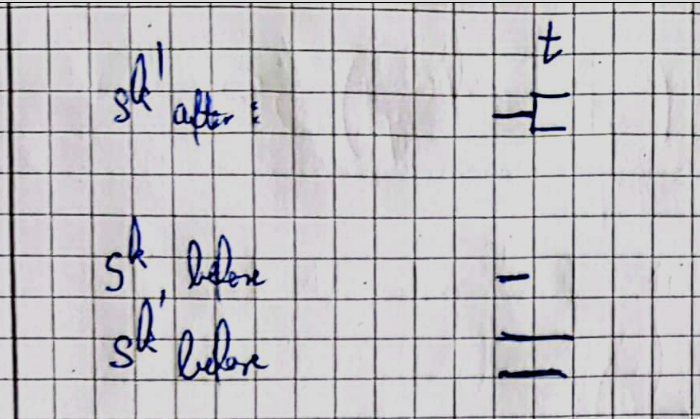
\includegraphics[width=0.5\textwidth]{graphics/sketches/activations.png}\label{fig:activations}
    \caption{}
  \end{figure}

  If $t \in V$, then processor $k' + 1$ (or $k$) must have been busy before at $t$.
  Hence $t$ was already an activation before the close, contradicting our initial choice of $t$.

  If $t \notin V$, then $t \succ V$.
  Let $W$ be the valley such that $V$ is closed during $\fillop(k, W)$, hence $W \supset V$.
  If $t \in W$, then $t \sim C_W$ and $t \in C_W$.
  By Invariant 2, processors $1, \ldots, k_W = k$ are busy at $t$ before the close.
  Again, this implies that $t$ was an activation before the close already, contradicting our choice of $t$.
  If $t \notin W$, then let $W'$ be the valley with $t \sim W$ and $t \in W'$.
  We have $W \prec t \sim W'$ and $W' \supset W$ and $t \in C_{W'}$.
  Therefore $k_{W'} \geq k_W = k$ and Invariant 2 implies that processors $1, \ldots, k$ are busy at $t$ before the close.
  Hence, $t$ was activation before the close already, again contradicting our initial choice of $t$.
\end{proof}
\begin{lemma}\label{lemma:constellation}
  Let $I$ an idle interval in $S_{real}$ on some processor $k$ and $A_l, A_r$ the busy intervals to the left and right of $I$ with $\crit(A_l) \leq 1$ and $\crit(A_r) \leq 1$.
  Allow $A_l$ to be empty, i.e.\ we might have $\min I = 0$, but $A_r$ must be nonempty, i.e.\ $\max I < d^*$.
  Then $k = 1$ and $\hat \phi(A_l \cup I \cup A_r) > 0$.
\end{lemma}
\begin{proof}
  By Lemma~\ref{lemma:activations} and $\crit(A_r) \leq 1$, we know that $\min A_r$ is an activation of processor $1$ in $S_{\aug}$.
  Hence $\max I$ is idle in $S_{\aug}$ on processor $1$ and hence on all processors (stair-property in $S_{\aug}$).
  Since no jobs are scheduled at $\max I$, we know that $\crit(\max I) \leq 1$ and $J_V = \emptyset$ for all valleys $V$ containing the slot $\max I$, and hence also $\res(V) = 0$ at all times during the realignment.
  Therefore, no $V$ intersecting $[\max I, \max A_r]$ was closed during realignment on any processor, since this $V$ would contain $\max I$.
  Since $A_r$ is a busy interval with $\crit(A_r) \leq 1$ (i.e.\ not containing activations of processors above $1$ in $S_{\aug}$), we must then have $k = 1$.

  For $I$ to be idle on processor $k = 1$ in $S_{\real}$ and $\crit(I) \geq 2$, some $V \succeq I$ with $V \cap I \neq \emptyset$ and hence $V \supseteq \max I$ would have to been closed, which contradicts what we have just shown.
  Therefore $\crit(I) \leq q$ and no valley $V$ with $V \cap [\min A_l - 1, \max A_r + 1] \neq \emptyset$ can have been closed.
  \todo{Properly define what `the constellation occurs in the same way in $S_{\aug}$` means.}
  Therefore, the constellation occurs exactly in the same way in $S_{\aug}$ on processor $1$, see Figure~\ref{fig:constellation}.

  \begin{figure}[H]
    \centering
    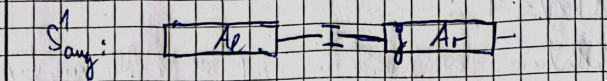
\includegraphics[width=0.6\textwidth]{graphics/sketches/constellation.png}\label{fig:constellation}
    \caption{}
  \end{figure}
  Let $j$ be the single job scheduled at $\min A_r$.
  We conclude by showing that $E_j \subseteq I \cup A_r$ and therefore $\hat \phi(I \cup A_r) > 0$.
  Otherwise, $j$ could be scheduled at $\min I$ or $\max A_r + 1$.
  In the first case, $\pltr$ would have extended $A_l$ by scheduling $j$ at time $\min I$ instead of at $\min A_r$.
  In the second case, $\pltr$ would have extended the idle interval $I$ by scheduling $j$ at $\max A_r + 1$ intead of at $\min A_r$.
\end{proof}

\begin{lemma}\label{lemma:intersection}
  For every processor $k$, every idle interval on processor $k$ in $S_{\opt}$ intersects at most two distinct idle intervals of processor $k$ in $S_{\real}$.
\end{lemma}
\begin{proof}
  Let $I_{\opt}$ be an idle interval in $S_{\opt}$ on processor $k$ intersecting three distinct idle intervals of processor $k$ in $S_{real}$.
  Let $I$ be the middle of these idle intervals.
  Lemma~\ref{lemma:constellation} and Lemma~\ref{lemma:phi_prop} imply that $k$ busy processors are required during $I$ and its neighboring busy intervals.
  This makes it impossible for $S_{\opt}$ to be idle on processor $k$ during the whole interval $I_{\opt}$.
  \todo{Sketch this}
\end{proof}

\subsection{Approximation Guarantee}
\begin{lemma}\label{lemma:costs_s_real}
  $\costs(S_{real}) \leq 2 \OPT + P$
\end{lemma}
\begin{proof}
  We first show that $\idle(S^k_{\real}) \leq 2 \off(S^k_{\opt}) + \on(S^k_{\opt})$ for every processor $k \in [m]$.
  Let $mathcal{I}_1$ be the set of idle intervals on $S^k_{real}$ intersecting some $\off$-interval of $S^k_{\opt}$.
  Lemma~\ref{lemma:intersection} implies that $\mathcal{I}_1$ contains as most twice as many intervals as there are $\off$-intervals in $S^k_{\opt}$.
  Therefore, the costs of these idle intervals is bounded by $2 \off(S^k_{\opt})$.

  Let $\mathcal{I}_2$ be the set of idle intervals on $S^k_{\real}$ not intersecting any $\off$-interval in $S^k_{\opt}$.
  The total length of these intervals is bounded by $\on(S^k_{\opt})$.

  We continue by showing that $\busy(S_{real}) \leq 2 P$.
  By construction of $S_{\aug}$ and the definition of $\res$ and $\close$, we introduce at most as many auxiliary busy slots at every slot $t \in T$ as there are jobs scheduled at $t$ in $S_{\pltr}$:
  For $S_{\aug}$, an auxiliary busy slot is only added for $t$ with $\crit(t) \geq 2$ and hence $\vol(t) \geq 1$.
  Furthermore, initially $\res(V) = 2 |J_V|$ for every valley $V$ and $\res(V)$ is decremented if some $V'$ intersecting $V$ is closed during $\fillop(k, T)$.
  During $\fillop(k, T)$ every $t \in T$ is at most closed once (or rather one $V'$ containing $t$ is closed).
  Finally, auxiliary busy slots introduced by $S_{\aug}$ are used in $\close$.
  In conclusion, we have $\costs(S_{\real}) \leq 2 \off(S_{\opt}) + \on(S_{\opt}) + 2 P \leq 2 \OPT + P$.
\end{proof}


\begin{theorem}
  $\costs(S_{\pltr}) \leq 2 \OPT + P$
\end{theorem}
\begin{proof}
  We argue that $\costs(S_{\pltr}) \leq \costs(S_{\real})$.
  The theorem then follows from Lemma~\ref{lemma:costs_s_real}.
  We do this by transforming $S_{\real}$ back into $S_{\pltr}$ without increasing the costs of the schedule.
  Removing the auxiliary busy slots clearly cannot increase the costs.
  Since the realignment of $S_{\aug}$ only moves busy slots between processors, but not between different time slots, we can easily restore $S_{\pltr}$ (up to permutations of the jobs scheduled on the busy processors at the same time slot) by moving all busy slots back down to the lower numbered processors.
  \todo{Define Lemma stair property somewhere}
  By the same argument as in Lemma~\ref{lemma:stair_property_opt}, this does not increase the total costs of the schedule.
\end{proof}

\section{Running Time}
\begin{theorem}
  Algorithm $\pltr$ has a running time of $O(F n \log d)$, where $F$ is the time needed for the flow calculation in Figure~\ref{fig:flow}.
\end{theorem}
\begin{proof}
  First observe that every busy interval is created by a pair of calls to $\keepidle$ and $\keepbusy$.
  Every call to $\keepidle$ searches for the maximal slot $t \in T$ (after the current time slot) such that the maximum-flow calculation in Figure~\ref{fig:flow} returns a flow of value $P$.
  Using binary search this can be done in $O(F \cdot \log(d^*))$ with $F$ denoting the time required for finding the maximum flow.

  We bound the number of busy intervals across all processors in $S_{\pltr}$ by $n$.
  Note that if $\keepidle$ returns $d^*$, then we do not have to calculate $\keepbusy$ from $d^*$ on.
  Therefore, the total number of calls to $\keepidle$ and $\keepbusy$ is bounded by $n + m$.
  If $m > n$ we can restrict our algorithm to use the first $n$ processors only, as there cannot be more than $n$ processors scheduling jobs at the same time.
  We derive the upper bound of $n$ for the number of busy intervals across all processors by constructing an injective mapping $f$ from the set of busy intervals to the jobs $J$.
  For this construction of $f$ we consider the busy intervals in the same order as the algorithm, i.e.\ from Top-Left to Bottom-Right.
  We construct $f$ such that $f(A) = j$ for some busy interval $A$ only if $d_j \in A$.

  Suppose we have constructed such a partial mapping for busy intervals on processors $m, \ldots, k$ up to some busy interval $A$ on $k$.
  \todo{Define plateaus: busy intervals which are completely idle on higher processors}
  Let $A'$ be the last plateau with $A' \subseteq A$ and let $k' \geq k$ be the processor of this plateau $A'$.
  By construction of $f$ and the choice of $A'$, there are at most $k' - (k + 1)$ distinct jobs $j$ with $d_j \in [\min A', \max A]$ already mapped to by $f$.
  This is since at most $k' - (k+1)$ busy intervals on processors $k+1, \ldots, m$ intersect the interval $[\min A', \max A]$.
  Refer to Figure~\ref{fig:running_time} for a visaul sketch.

  \begin{figure}[H]
    \centering
    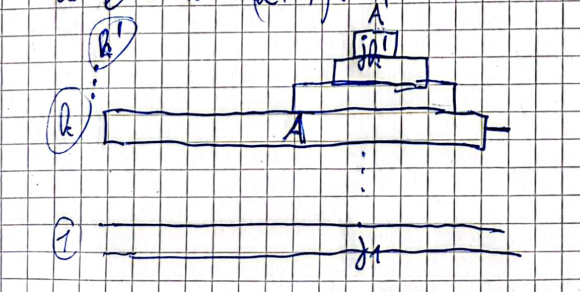
\includegraphics[width=0.5\textwidth]{graphics/sketches/running_time.png}\label{fig:running_time}
    \caption{}
  \end{figure}

  Let $C_t$ be the critical set over activation $t \coloneqq \min A'$ of processor $k'$.
  Let $J' \coloneqq \{ j_1, \ldots, j_{k'} \}$ be the $k'$ distinct jobs scheduled at $t$.
  We now that $\max A + 1 \notin C_t$ since $\vol(\max A + 1) < k \leq k'$ and $\max A + 1 > t$.
  Therefore, every job $j \in J'$ with $d_j \geq \max A + 1$ is scheduled at slot $\max A + 1$.
  Hence there are at least $k' - (k-1)$ distinct jobs $j \in J'$ with $d_j \in [\min A', \max A]$ and there must be at least one such job $j^*$ which is not mapped to by $f$ so far and which we therefore can use for $f(A)$.
\end{proof}
%\bibliographystyle{plain}
\bibliographystyle{abbrvnat}
%\setcitestyle{authoryear,open={(},close={)}}
\bibliography{references}
\end{document}
